\section{Integrated Gradients}


\begin{figure*}
    \centering
    \begin{subfigure}{\textwidth}
        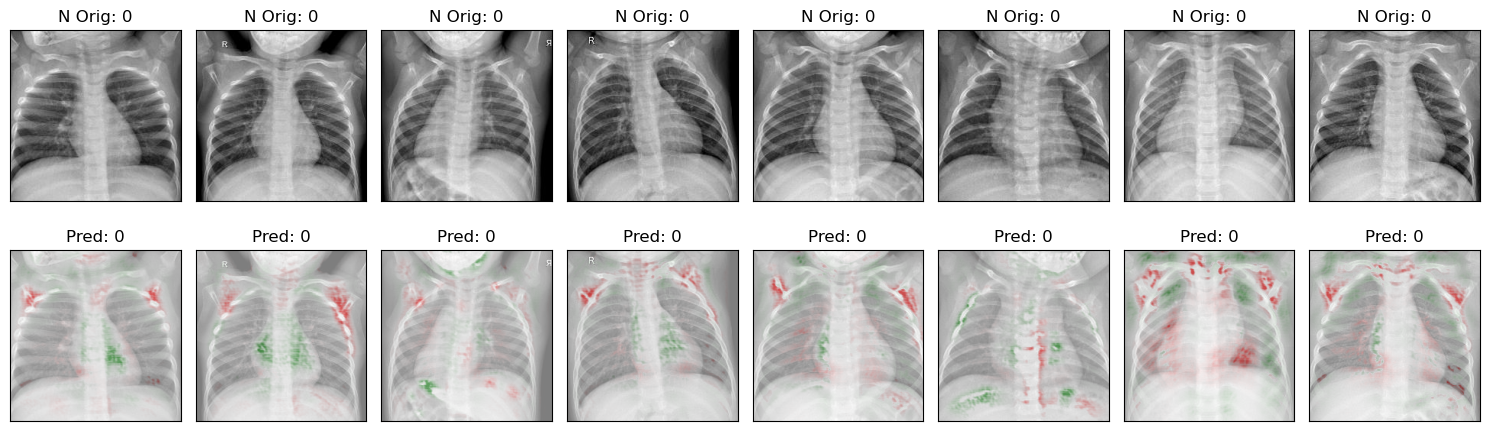
\includegraphics[width=1\textwidth]{images/IG_train.png}
    \end{subfigure}
    \centering
    \begin{subfigure}{\textwidth}
        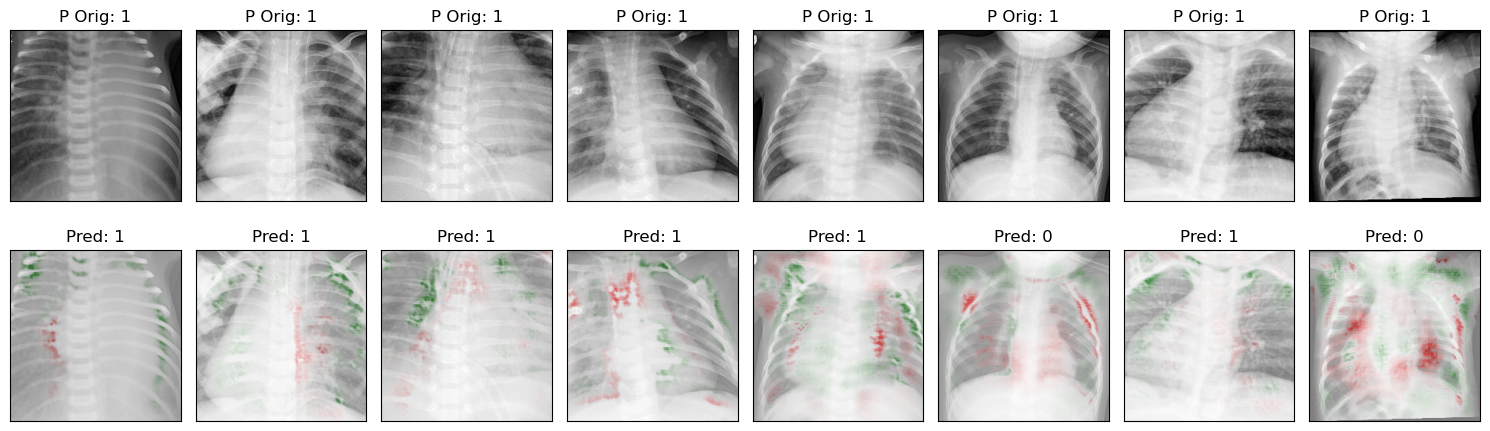
\includegraphics[width=1\textwidth]{images/IG_train_P.png}
    \end{subfigure}
    \caption{Training images to which integrated gradients was applied. Upper two rows are from healthy patients, bottom two rows from patients with pneumonia. The 1st and 3rd row contain the input image, the 2nd and 4th row contain an added overlay from integrated gradients. In red is the negative attribution, in green the positive attribution.}
    \label{fig:ig_train}
\end{figure*}

Integrated gradients (IG) applied to images allows us to attribute a certain importance to each pixel. This importance can be negative, i.e. this pixel makes the prediction for the class that is currently being looked at less likely, but also positive, i.e. this pixel positively contributes to the prediction of that class.

For applying the integrated gradients method, we adapt the code from \cite{alibi} and calculate the gradient along the path between the given image and a black 'baseline' image. We choose an all-zeros baseline image because the background of an X-ray image is also black, and signifies the 'absence of signal'. This is deemed important in the original paper from Sundararajan et al. \cite{ig}.

We use the trapezoidal version of Riemann gradient approximation, as this seems to be what \cite{ig} mentions.

\subsection*{A. Visualization}

As you can see in Figure \ref{fig:ig_train}, the main focus point for most patients, both healthy and sick, is the bones in the shoulder and the outer contours of the upper ribs. For healthy patients, this is considered a negative attribute, for sick patients a positive one.

In addition, some attention is paid to the areas where the airways branch out, near the center of the image (i.e. near the hilums of the lungs). This makes sense, since sick patients often have increased thickening of the smaller airways.

In some images, we are also able to observe focus on the spaces in between the ribs, which seems to be a sensible place to look, since that's where we can see the lungs and its contents the best.

The reason why the model seems to focus on the chin, might be due to its ability to look for enlarged lymph nodes in the throat area, since the pneumonia might have been preceded by a throat infection.

Overall, the model is focusing a lot on bones, but this could be contributed to the fact that the shoulders in healthy patients are often included in the X-ray, while this does not seem to happen as often for patients with pneumonia. Perhaps it was more difficult to keep a sick child still during the imaging, as compared to healthy children, and therefore the parents' help was needed to 'pin' the sick children down (maybe holding their head still with their hands), which caused the image to not include the lower part of the head and upper part of the shoulders. This is just a hypothesis of course.

The results for the test set in Figure \ref{fig:ig_test} largely confirm what is seen in the training data, although the shoulders seem to be detected more often for sick patients.

\begin{figure}
    \centering
    \begin{subfigure}{\columnwidth}
        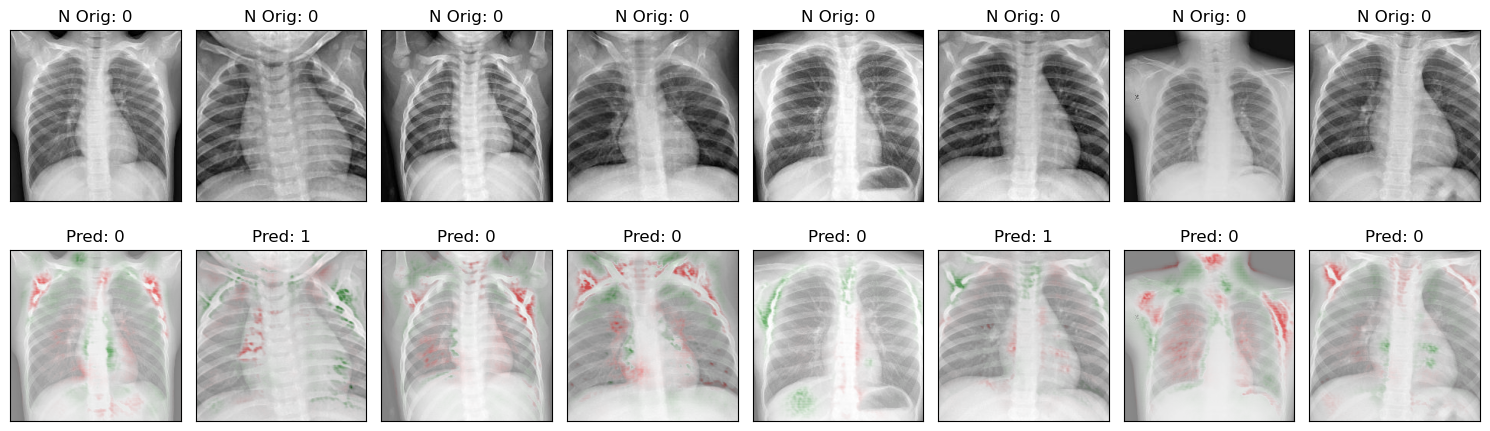
\includegraphics[width=1\textwidth]{images/IG_test.png}
    \end{subfigure}
    \centering
    \begin{subfigure}{\columnwidth}
        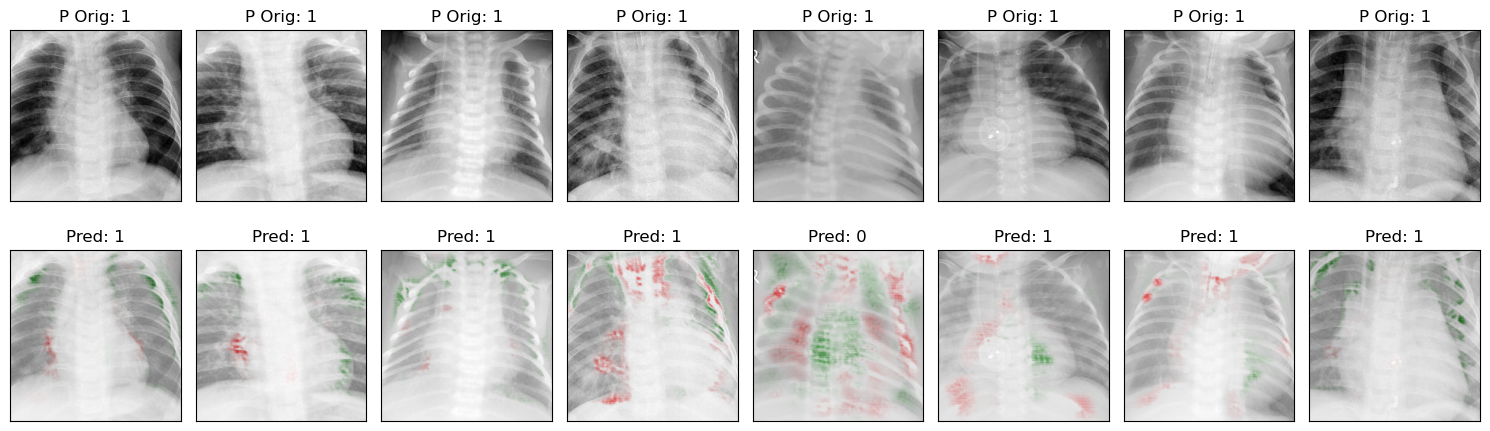
\includegraphics[width=1\textwidth]{images/IG_test_P.png}
    \end{subfigure}
    \caption{Test images to which integrated gradients was applied. Upper two rows are from healthy patients, bottom two rows from patients with pneumonia. The 1st and 3rd row contain the input image, the 2nd and 4th row contain an added overlay from integrated gradients. In red is the negative attribution, in green the positive attribution.}
    \label{fig:ig_test}
\end{figure}